\section*{Figures}


\begin{verbatimwrite}{./Slides/FigureParker}%%%Slides
\begin{figure}[!ht] \centering  % [h!]
	\caption{ ~Portfolio responses to 2016 U.S. election}
	\label{fig:parker}
	\centerline{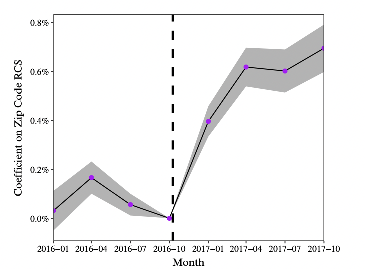
\includegraphics[width=\textwidth]{./figures/parker}}
	\begin{flushleft}
		{\footnotesize Note: reproduced from \cite{meeuwis2018belief}, this figure reports the baseline regression coefficients of equity share on zip-code level  campaign contribution share to Republican candidate for the three quarters prior to the election and the four quarters following the election, relative to allocations just before the election.}
	\end{flushleft}
\end{figure}
\end{verbatimwrite}%%%Slides
%%%Slides
  \begin{figure}[!ht] \centering  % [h!]
    \caption{ ~Portfolio responses to 2016 U.S. election}
    \label{fig:parker}
    \centerline{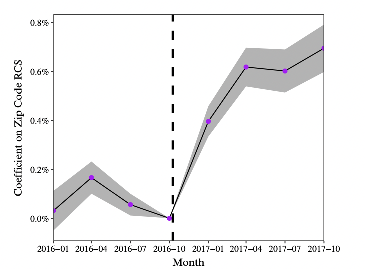
\includegraphics[width=\textwidth]{./figures/parker}}
    \begin{flushleft}
      {\footnotesize Note: reproduced from \cite{meeuwis2018belief}, this figure reports the baseline regression coefficients of equity share on zip-code level  campaign contribution share to Republican candidate for the three quarters prior to the election and the four quarters following the election, relative to allocations just before the election.}
    \end{flushleft}
  \end{figure}
%%%Slides



\begin{verbatimwrite}{./Slides/FigureSIRFlowDiagram}%%%Slides
\begin{figure}[!ht] \centering  % [h!]
	\caption{ ~A SIR model of stock investors}
		\label{fig:sir_diagram}
		\centerline{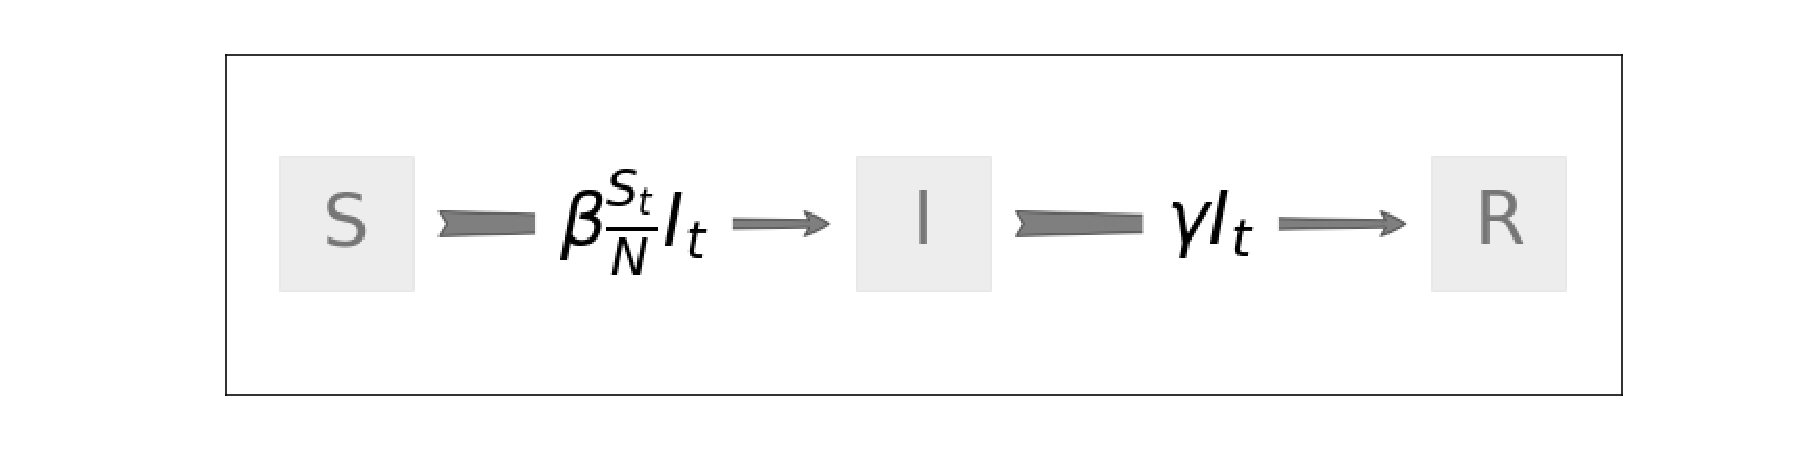
\includegraphics[width=\textwidth]{./figures/flow_diagram}}
		\begin{flushleft}
		{\footnotesize Note: This graph plots the transitions between different compartments in the SIR model of the stock investors as described in \cite{shiller1989survey}. }
			\end{flushleft}
	\end{figure}
\end{verbatimwrite}%%%Slides
%%%Slides
	\begin{figure}[!ht] \centering  % [h!]
		\caption{ ~A SIR model of stock investors}
		\label{fig:sir_diagram}
		\centerline{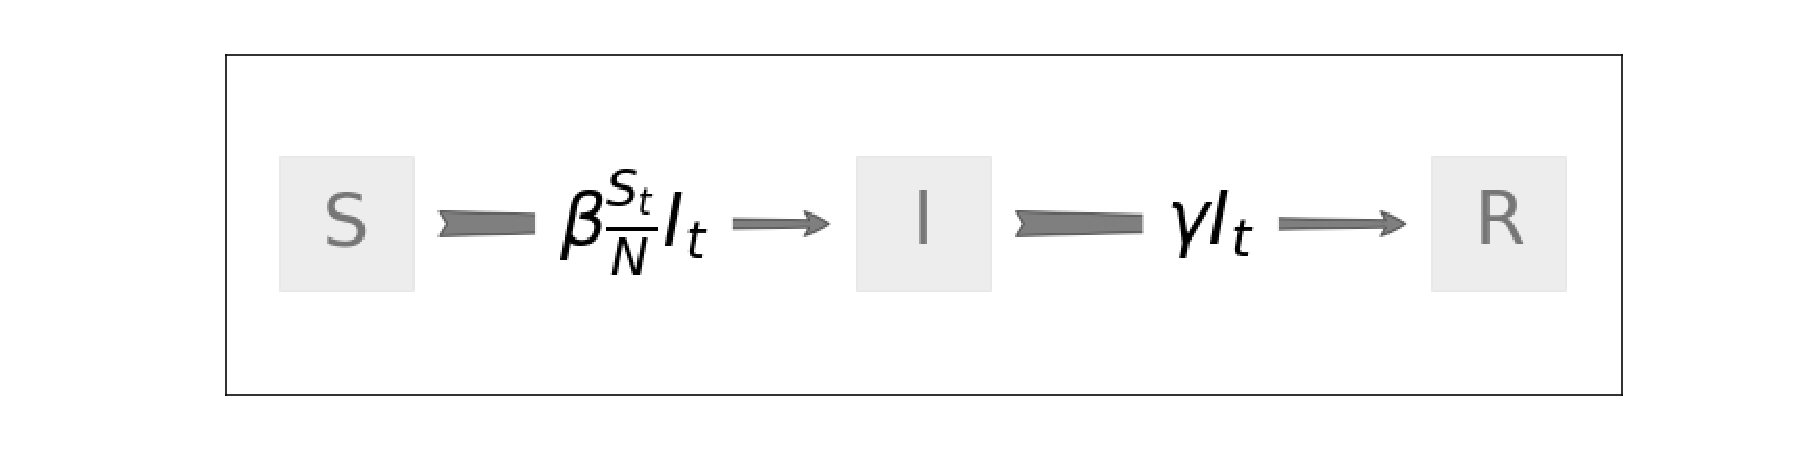
\includegraphics[width=1.5\textwidth]{./figures/flow_diagram}}
		\begin{flushleft}
			{\footnotesize Note: This graph plots the transitions between different compartments in the SIR model of stock investors described in \cite{shiller1989survey}. }
		\end{flushleft}
	\end{figure}


\newpage

\begin{verbatimwrite}{./Slides/FigureSIRSimulation}%%%Slides
\begin{figure}[!ht] \centering  % [h!]
	\caption{ ~Simulated dynamics from a SIR model of stock investors}
	\label{fig:sir_simulate}
	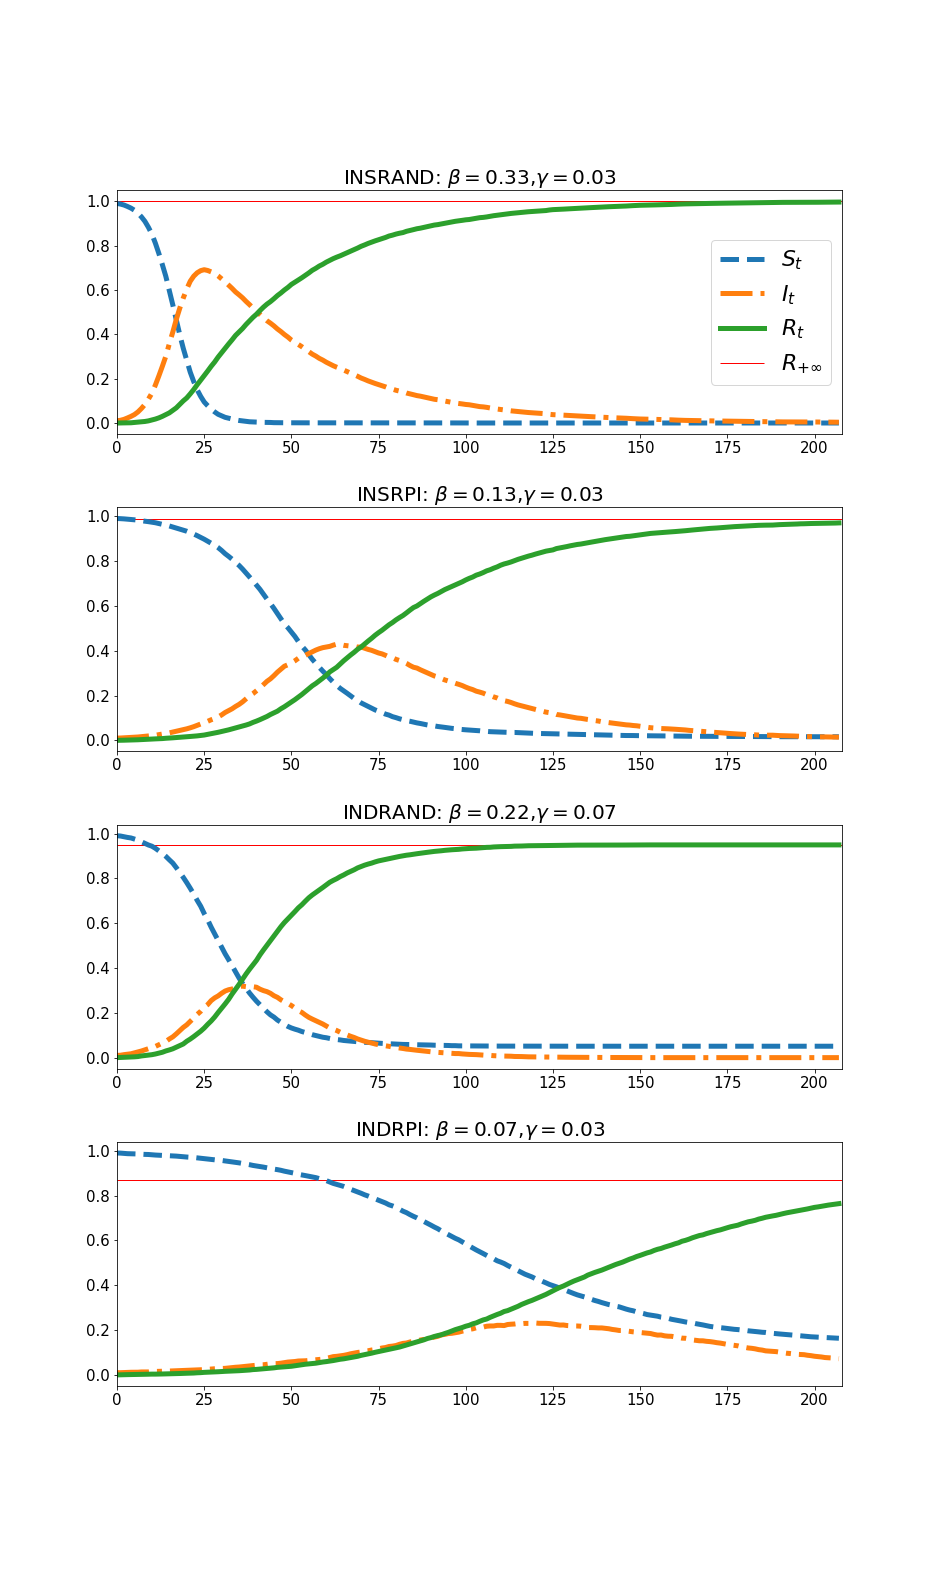
\includegraphics[width=0.85\textwidth,height=0.85\textheight]{./figures/sir_simulate}
	\begin{flushleft}
	{\footnotesize Note: This graph plots the simulated paths of populations in different compartments in a SIR model of stock investors, as described in \cite{shiller1989survey}. We use the median estimates of the infection rate $\beta$ and recovery rate $\gamma$ for four samples: institutional investors for a randomly selected stock (INSRAND), institutional investors for a rapidly rising stock (INSRPI), individual investors for a random stock (INDRAND), and individual investors for a rapidly rising stock (INDRPI). The horizontal dashed line corresponds to the limiting size of compartment of $R$ in the long run. The simulation is done with the Python library ``NDlib'', for details, see the companion \href{https://github.com/llorracc/EpiExp/blob/master/SIR_Ndlib.ipynb}{Jupyter Notebook}. }
				\end{flushleft}
\end{figure}
\end{verbatimwrite}%%%Slides
%%%Slides
  \begin{figure} \centering  % [h!]  [!ht]
    \caption{ ~Simulated dynamics from an SIR model of stock investors}
    \label{fig:sir_simulate}
    \centerline{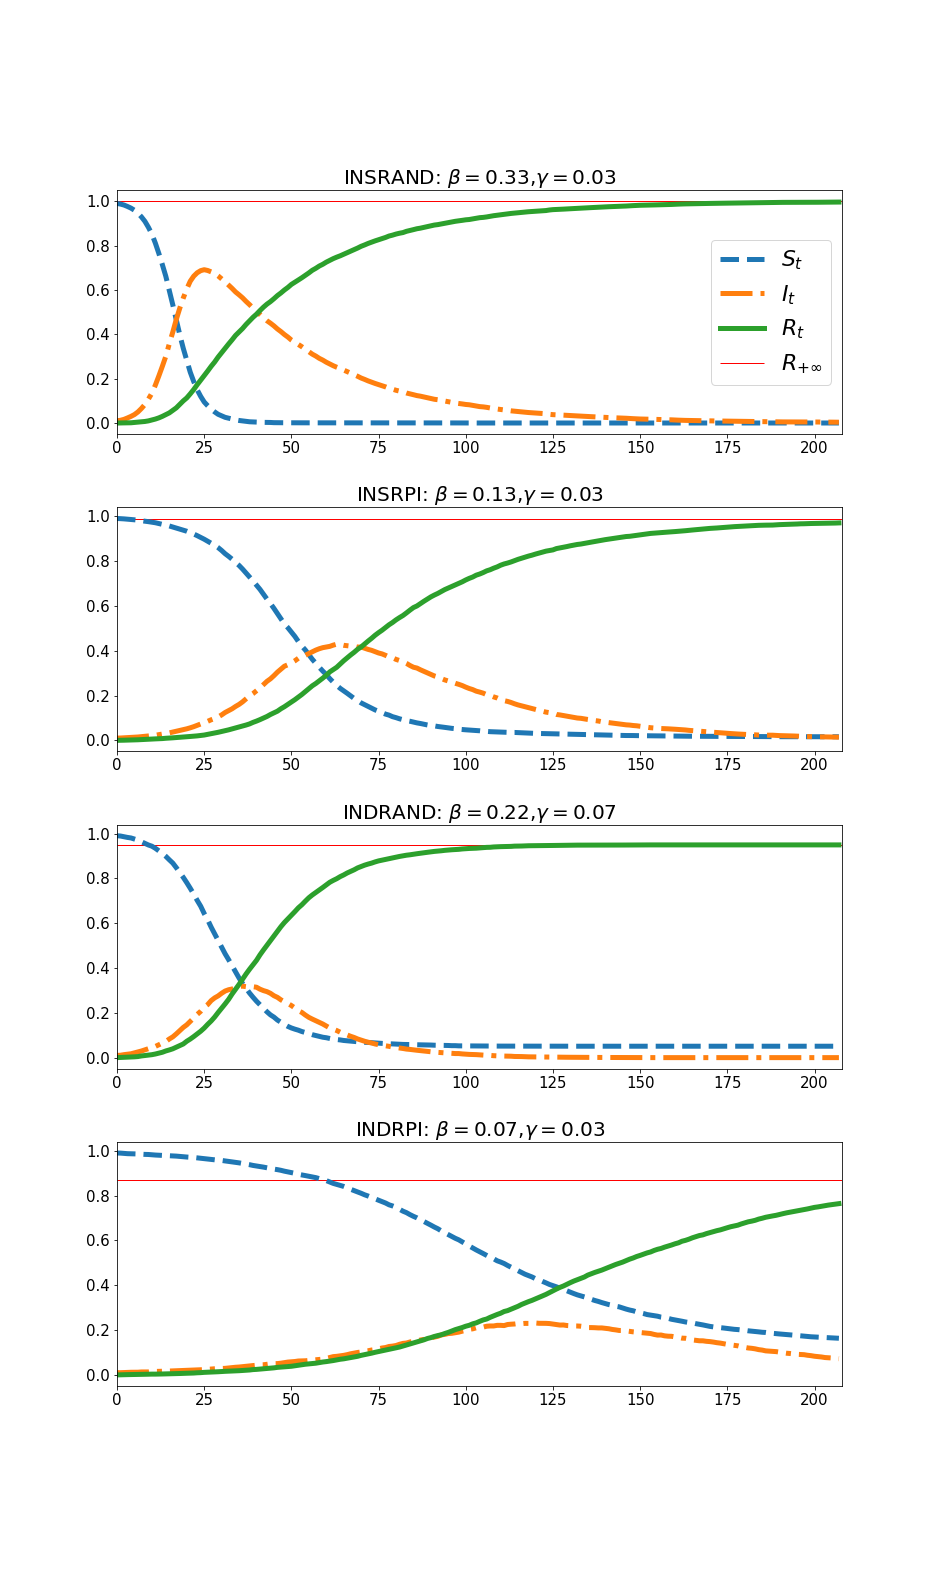
\includegraphics[width=0.85\textwidth,height=0.85\textheight]{./figures/sir_simulate}}
    \begin{flushleft}
      {\footnotesize Note: This graph plots the simulated paths of populations in different compartments in a SIR model of stock investors, as described in \cite{shiller1989survey}. We use the median estimates of the infection rate $\beta$ and recovery rate $\gamma$ for four samples: institutional investors for a randomly selected stock (INSRAND), institutional investors for a rapidly rising stock (INSRPI), individual investors for a random stock (INDRAND), and individual investors for a rapidly rising stock (INDRPI). The horizontal thin solid line corresponds to the limiting size of compartment of $R$ in the long run. The simulation is done with the Python library \href{https://ndlib.readthedocs.io/en/latest/}{``NDlib''}, for details, see the companion \href{https://github.com/llorracc/EpiExp/blob/master/SIR_Ndlib.ipynb}{Jupyter Notebook}. }
    \end{flushleft}
  \end{figure}
%%%Slides

\newpage

\begin{figure}[!ht] \centering  % [h!]
	\caption{ ~Literature map of cited papers}
	\label{fig:graph_mixer}
	\centerline{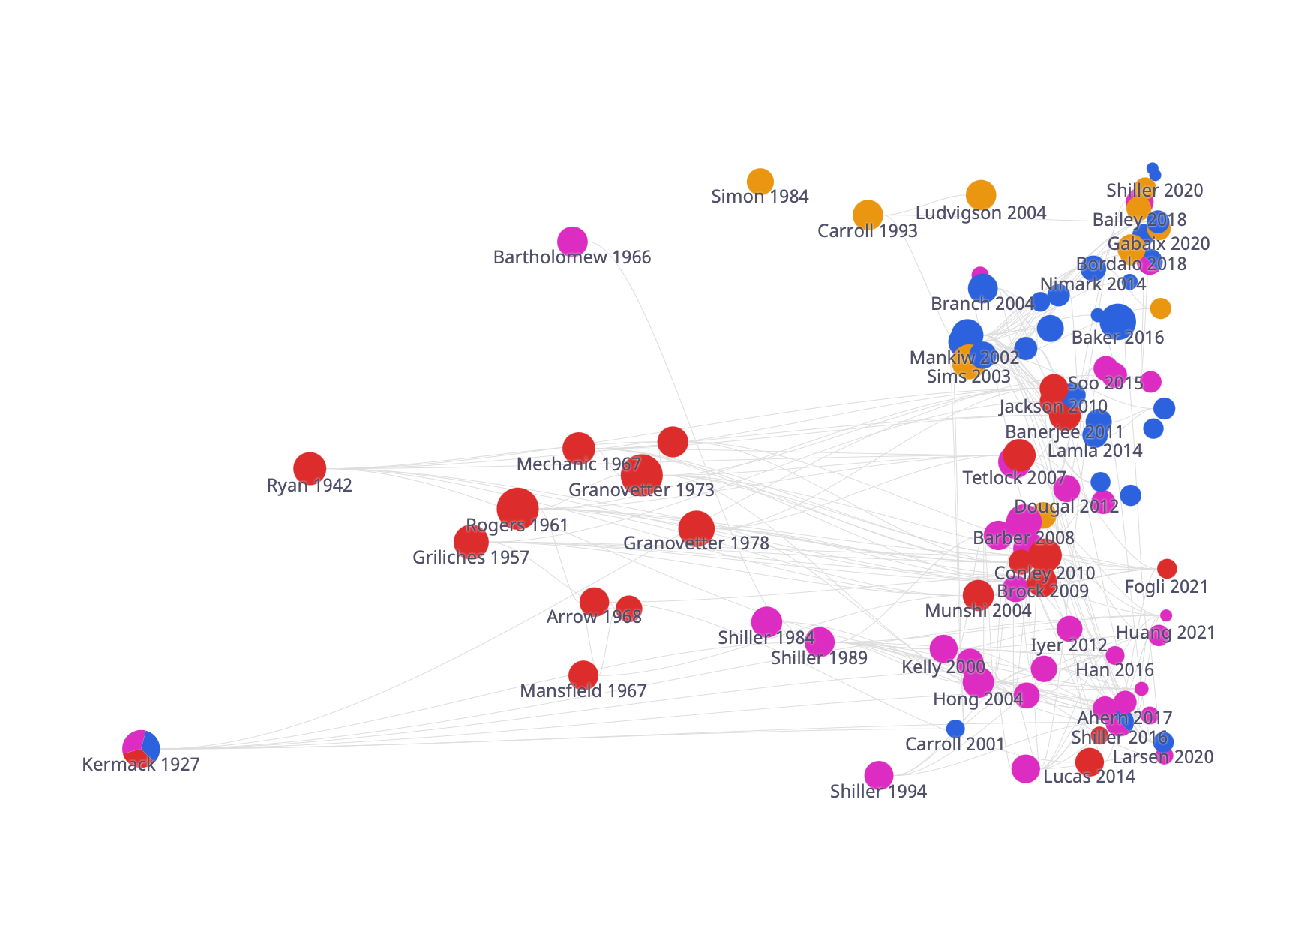
\includegraphics[width=\textwidth]{./figures/graph_mixer}}
	\begin{flushleft}
		{\footnotesize Note: This graph includes selected papers under three topics of epidemiological expectations: technological diffusion, asset market investment and macroeconomic expectations, represented by different color.  It also includes other papers we have cited because they have results likely to be interesing to EE modelers.}
	\end{flushleft}
\end{figure}

\newpage

\begin{figure}[!ht] \centering  % [h!]
	\caption{ ~Literature map of EE models of technological diffusion}
	\label{fig:graph_diffusion}
	\centerline{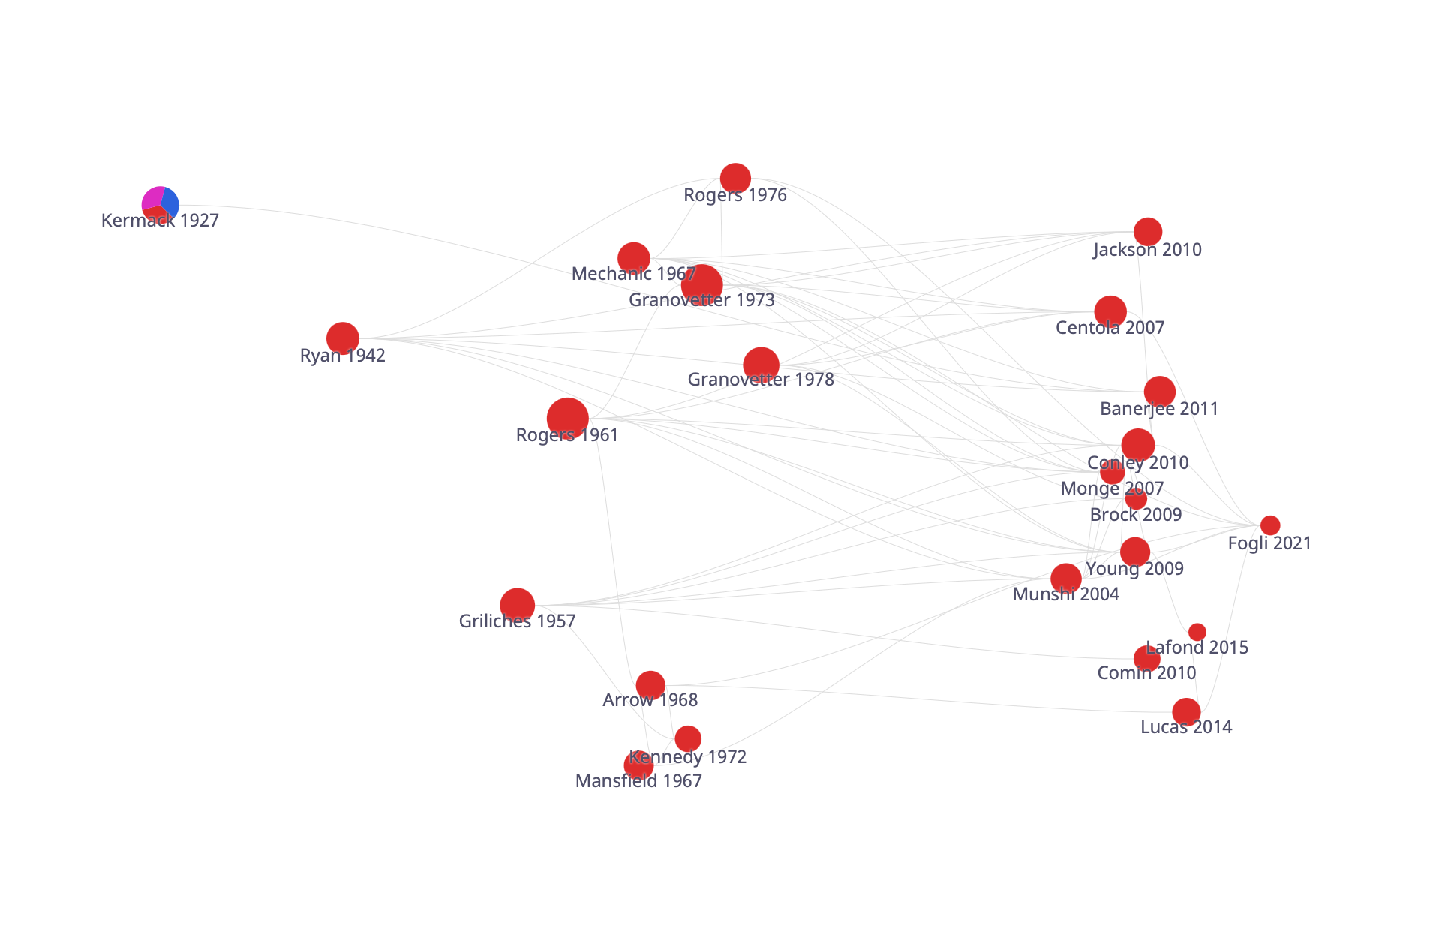
\includegraphics[width=\textwidth]{./figures/graph_diffusion}}
		\begin{flushleft}
{\footnotesize Note: This graph includes selected papers under the topic of epidemiological modeling of technological/innovation diffusion in economics and its related literature from other fields. See \href{https://app.litmaps.co/shared/1D9003CB-75FE-4633-B60A-79B70E03B691}{here} for its interactive version.}
				\end{flushleft}
\end{figure}

\newpage

\begin{figure}[!ht] \centering  % [h!]
	\caption{ ~Literature map of EE models of stock/housing market investment}
	\label{fig:graph_investment}
	\centerline{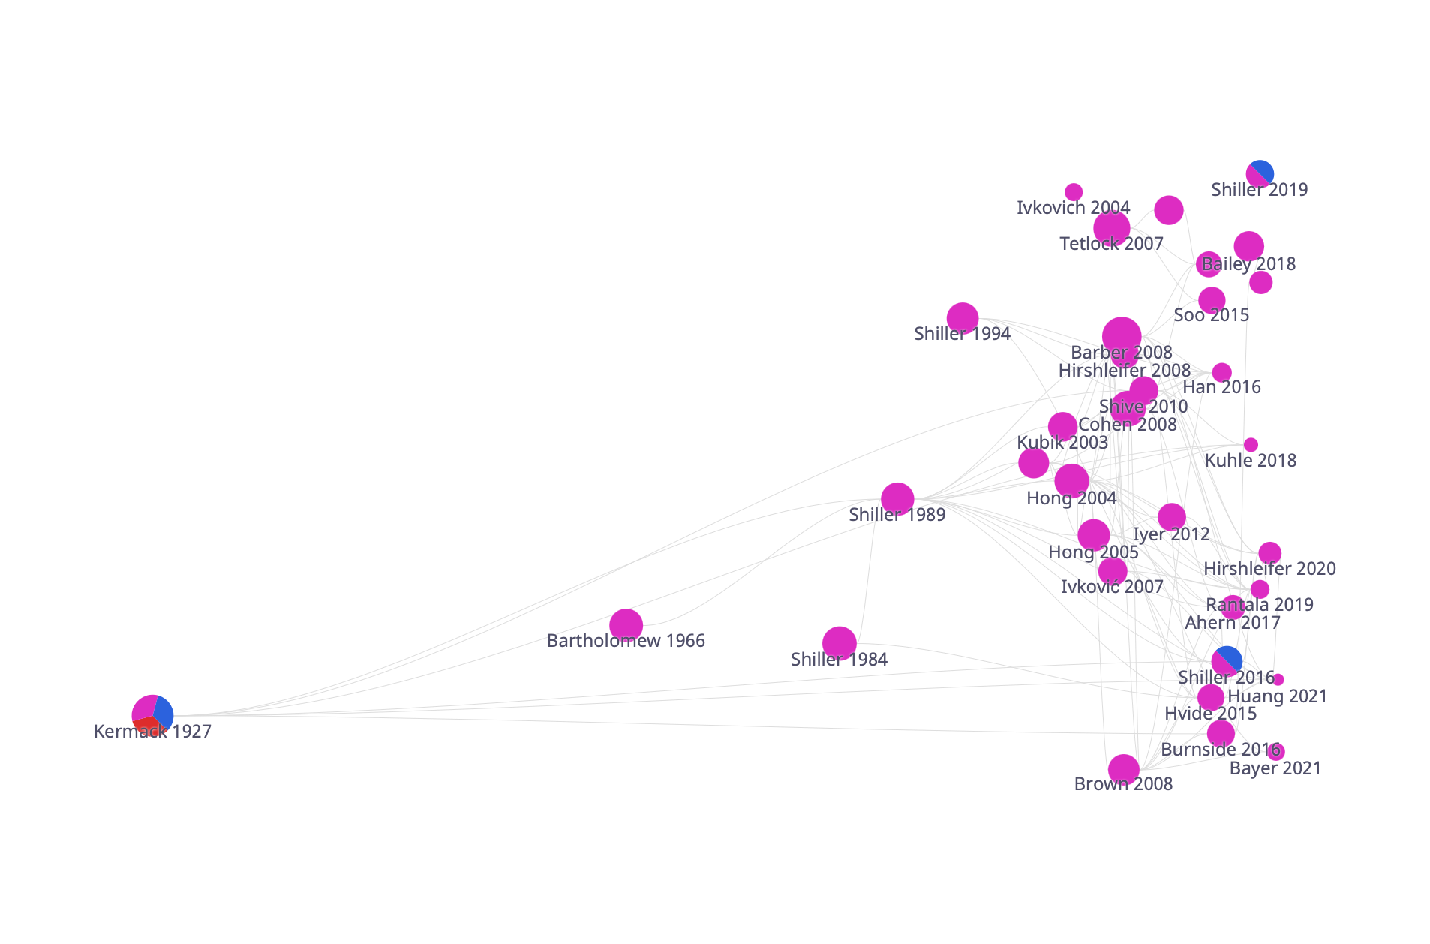
\includegraphics[width=\textwidth]{./figures/graph_investment}}
			\begin{flushleft}
	{\footnotesize Note: This graph includes selected papers related to epidemiological models of expectations in financial markets such as stocks and housing, and studies on the role of news media in financial markets. See \href{https://app.litmaps.co/shared/E25276CA-8725-437B-8241-11961EFB3FB4}{here} for its interactive version.}
					\end{flushleft}
\end{figure}

\newpage


\begin{figure}[!ht] \centering  % [h!]
    %\hypertarget{graphmacro}{}
		\caption{ ~Literature map of EE models of macroeconomic expectations}
	\label{fig:graph_macro}
	\centerline{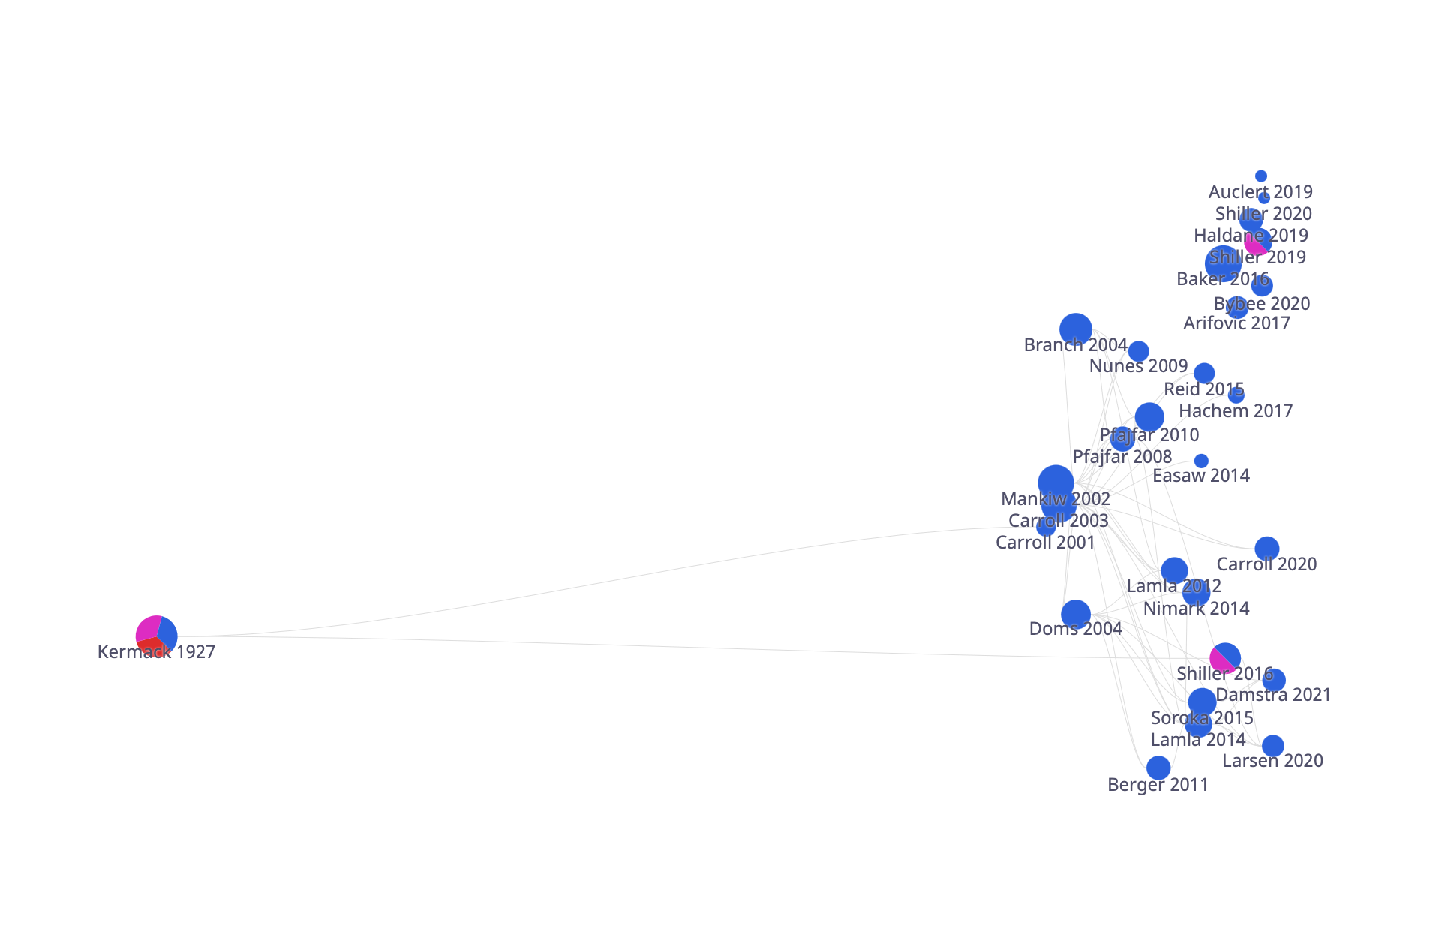
\includegraphics[width=\textwidth]{./figures/graph_macro}}
				\begin{flushleft}
		{\footnotesize Note: This graph includes selected papers related to epidemiological models of macroeconomic expectations, and research on the interaction between news media and macroeconomic expectations. See \href{https://app.litmaps.co/shared/289F57F4-FDE5-4F94-B1A9-2BA7419DB719}{here} for its interactive version.}
							\end{flushleft}
\end{figure}

\newpage

\begin{figure}[!ht] \centering  % [h!]
	\caption{ ~Other fields related to epidemiological models}
	\label{fig:graph_other}
	\centerline{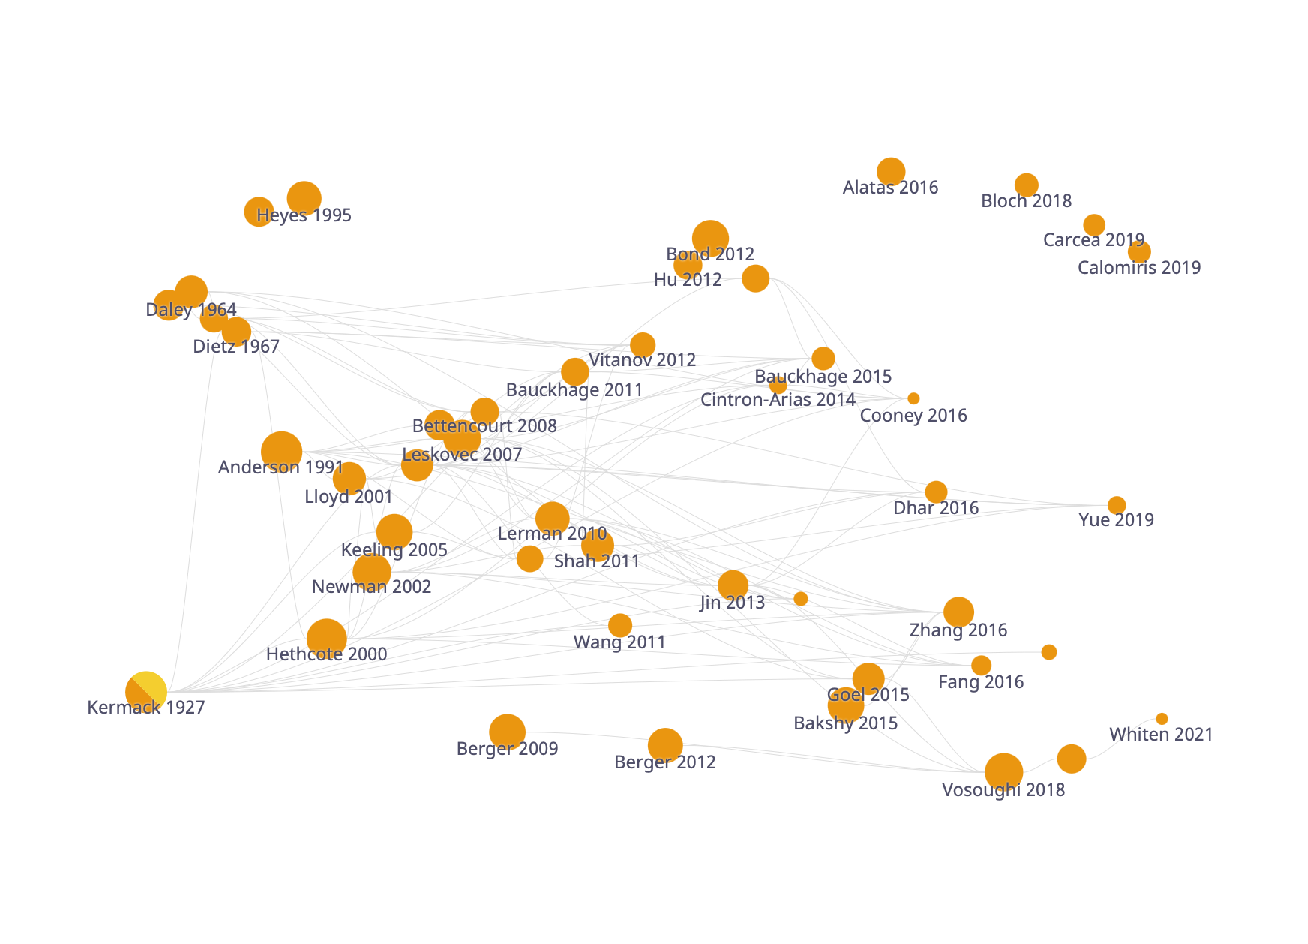
\includegraphics[width=\textwidth]{./figures/graph_other}}
				\begin{flushleft}{\footnotesize Note: This graph includes all other papers surveyed in this chapter. It includes epi models of rumor/news/online content/scientific ideas as well as other economic research on bank runs, herd behaviors, contagion, and peer effects. See \href{https://app.litmaps.co/shared/B5FA1F14-01A8-4C9D-BF23-BE0F62293FAF}{here} for its interactive version.}
						\end{flushleft}
\end{figure}


\newpage


\begin{verbatimwrite}{./Slides/FigureNewsCurve}
\begin{figure}[!ht] \centering  % [h!]
	\caption{ ~Spreading of news and rumors: \href{https://people.cs.vt.edu/ramakris/papers/news-rumor-epi-snakdd13.pdf}{Jin et al (2013)}}\nocite{jin2013epidemiological}
	\label{fig:news_curve}
	\centerline{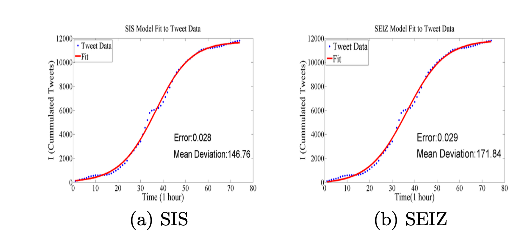
\includegraphics[width=\textwidth]{./figures/Doomsday}}
		\begin{flushleft}{\footnotesize Note: This graph is reproduced from \cite{jin2013epidemiological}, showing their fitted SIS and SEIZ model of the counts of Twitter posts related to the ``Doomsday'' rumor, which was widely circulated before December 21, 2012.}
	\end{flushleft}
\end{figure}
\end{verbatimwrite}%%%Slides
  \begin{figure}[!ht] \centering  % [h!]
    \caption{ ~Spreading of news and rumors: Jin et al (2013)}\nocite{jin2013epidemiological}
    \label{fig:news_curve}
    \centerline{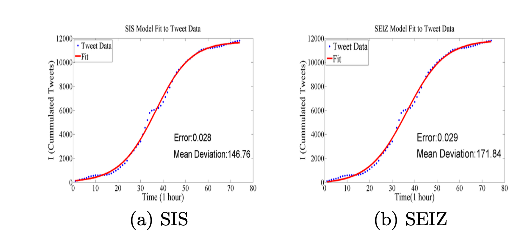
\includegraphics[width=\textwidth]{./figures/Doomsday}}
    \begin{flushleft}{\footnotesize Note: This graph is reproduced from \cite{jin2013epidemiological}, showing their fitted SIS and SEIZ model of the counts of Twitter posts related to the ``Mayan Doomsday'' rumor, which was widely circulated before December 21, 2012.}
    \end{flushleft}
  \end{figure}


\newpage


\begin{verbatimwrite}{./Slides/FigureScienceIdeasCurve}
\begin{figure}[!ht] \centering  % [h!]
	\caption{ ~Diffusion of scientific ideas: \href{http://web.mit.edu/dikaiser/www/BAKC.PhysA.pdf}{Bettencourt et al (2006)}}\nocite{bettencourt2006power}
	\label{fig:science_ideas_curve}
	\centerline{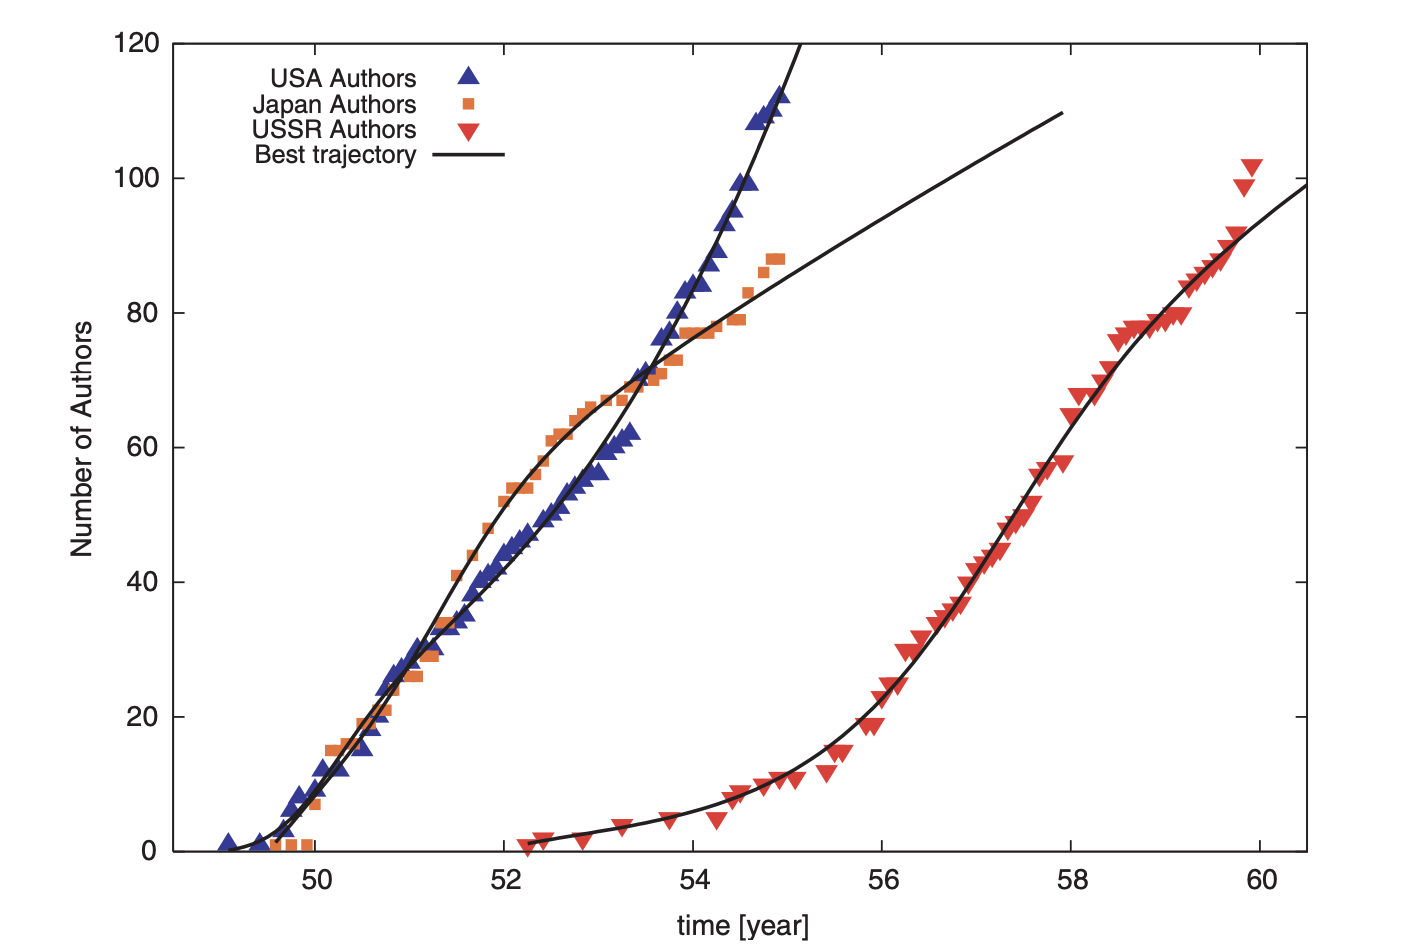
\includegraphics[width=\textwidth]{./figures/Feynman}}
		\begin{flushleft}{\footnotesize Note: This graph is reproduced from \cite{bettencourt2006power}, showing their fitted SEIZ model to the diffusion dynamics of Feynman diagrams in three theoretical physics communities, measured by the cumulative number of authors using the Feynman diagrams.}
	\end{flushleft}
\end{figure}
\end{verbatimwrite}%%%Slides
	\begin{figure}[!ht] \centering  % [h!]
		\caption{ ~Diffusion of scientific ideas: \href{http://web.mit.edu/dikaiser/www/BAKC.PhysA.pdf}{Bettencourt et al (2006)}}\nocite{bettencourt2006power}
		\label{fig:science_ideas_curve}
		\centerline{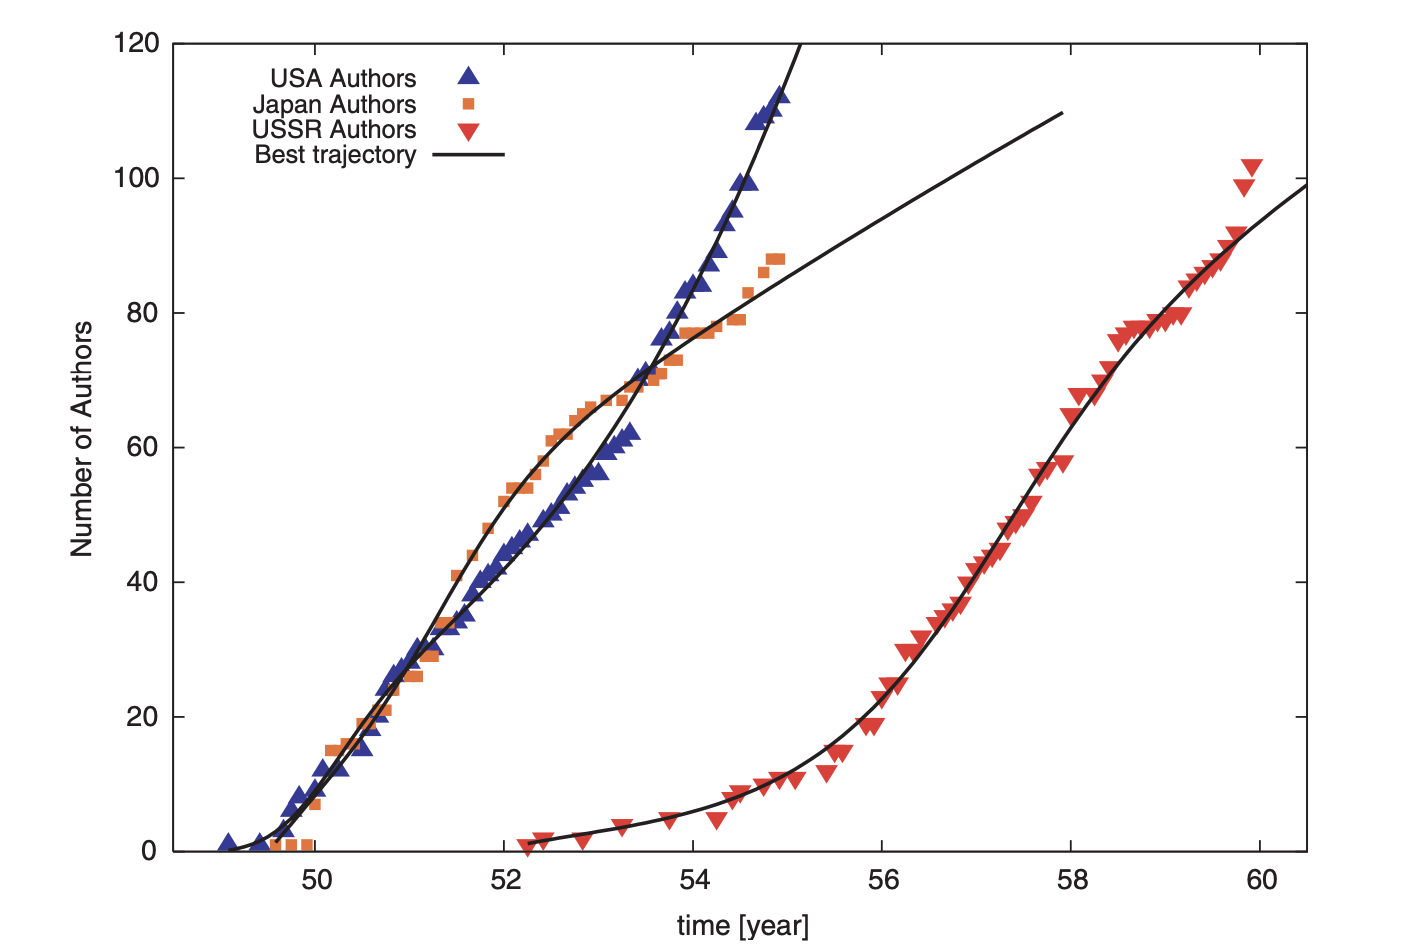
\includegraphics[width=\textwidth]{./figures/Feynman}}
		\begin{flushleft}{\footnotesize Note: This graph is reproduced from \cite{bettencourt2006power}, showing their fitted SEIZ model to the diffusion dynamics of Feynman diagrams in three theoretical physics communities, measured by the cumulative number of authors using the Feynman diagrams.}
		\end{flushleft}
	\end{figure}


\newpage

\begin{verbatimwrite}{./Slides/FigureMemesCurve}
\begin{figure}[!ht] \centering  % [h!]
	\caption{ ~Virality of internet memes: \href{https://github.com/iworld1991/EpiExp/blob/master/Literature/bauckhage2011insights.pdf}{\cite{bauckhage2011insights}}}
	\label{fig:memes_curve}
	\centerline{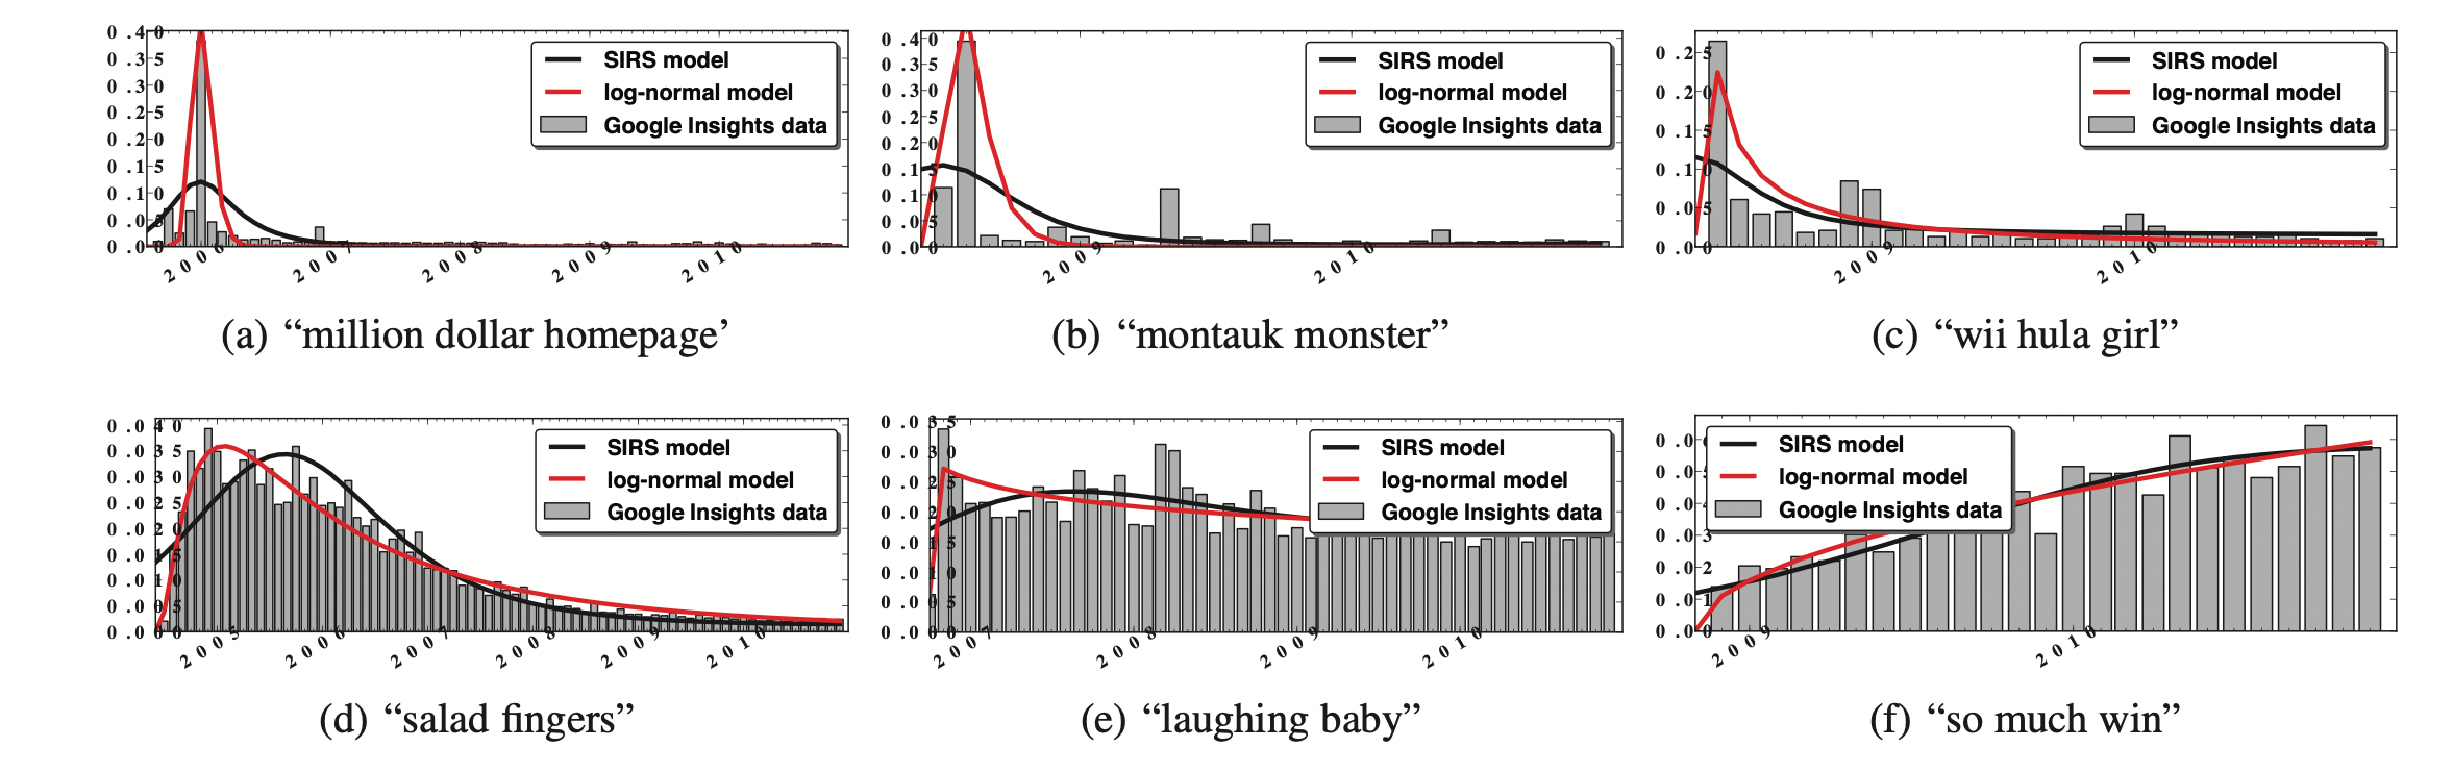
\includegraphics[width=\textwidth]{./figures/Memes}}
	\begin{flushleft}{\footnotesize Note: This graph reproduces the SIRS model fit and log-normal fits to Google insights time series measuring the interest in six viral memes, as shown in  \cite{bauckhage2011insights}. }
\end{flushleft}
\end{figure}
\end{verbatimwrite}%%%Slides
{figure}[!ht] \centering \caption { ~Virality of internet memes: \href {https://github.com/iworld1991/EpiExp/blob/master/Literature/bauckhage2011insights.pdf}{\cite {bauckhage2011insights}}} \label {fig:memes_curve} \subfloat [``salad fingers'']{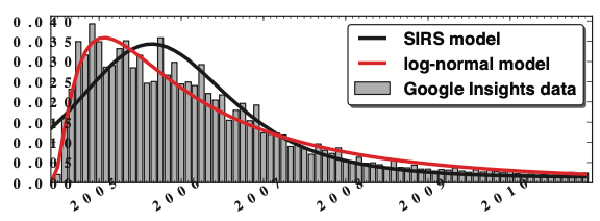
\includegraphics [width=\textwidth ]{./figures/Memes1}} \newline \subfloat [``laughing baby'']{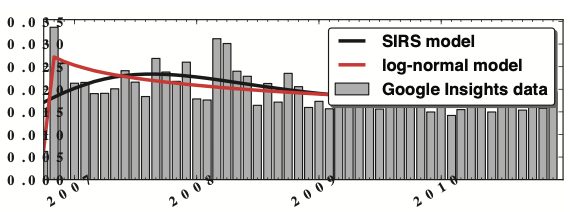
\includegraphics [width=\textwidth ]{./figures/Memes2}} \newline \subfloat [``so much win'']{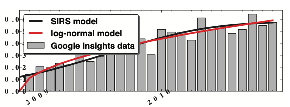
\includegraphics [width=\textwidth ]{./figures/Memes3}} \begin {flushleft}{\footnotesize Note: This graph reproduces the SIRS model fit and log-normal fits to Google insights time series measuring the interest in six viral memes, as shown in \cite {bauckhage2011insights}. } \end {flushleft} \end {figure} \end {verbatimwrite}{figure}[!ht] \centering \caption { ~Virality of internet memes: \href {https://github.com/iworld1991/EpiExp/blob/master/Literature/bauckhage2011insights.pdf}{\cite {bauckhage2011insights}}} \label {fig:memes_curve} \subfloat [``salad fingers'']{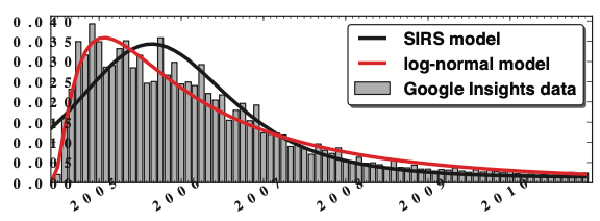
\includegraphics [width=\textwidth ]{./figures/Memes1}} \newline \subfloat [``laughing baby'']{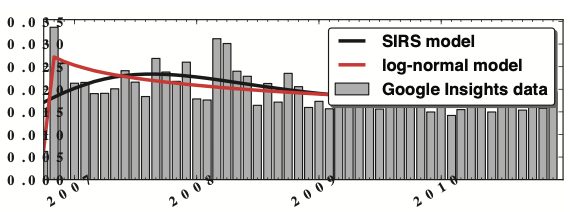
\includegraphics [width=\textwidth ]{./figures/Memes2}} \newline \subfloat [``so much win'']{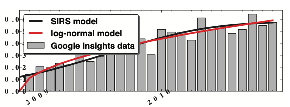
\includegraphics [width=\textwidth ]{./figures/Memes3}} \begin {flushleft}{\footnotesize Note: This graph reproduces the SIRS model fit and log-normal fits to Google insights time series measuring the interest in six viral memes, as shown in \cite {bauckhage2011insights}. } \end {flushleft} \end {figure} \end {verbatimwrite}{figure}[!ht] \centering \caption { ~Virality of internet memes: \href {https://github.com/iworld1991/EpiExp/blob/master/Literature/bauckhage2011insights.pdf}{\cite {bauckhage2011insights}}} \label {fig:memes_curve} \subfloat [``salad fingers'']{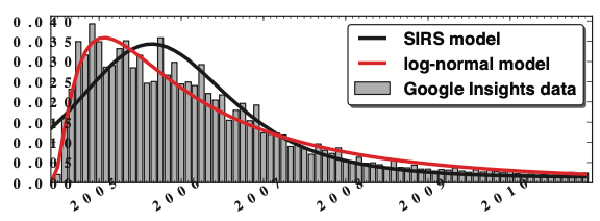
\includegraphics [width=\textwidth ]{./figures/Memes1}} \newline \subfloat [``laughing baby'']{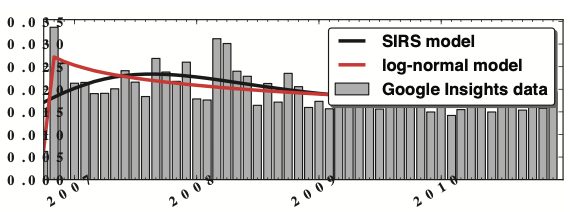
\includegraphics [width=\textwidth ]{./figures/Memes2}} \newline \subfloat [``so much win'']{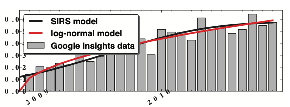
\includegraphics [width=\textwidth ]{./figures/Memes3}} \begin {flushleft}{\footnotesize Note: This graph reproduces the SIRS model fit and log-normal fits to Google insights time series measuring the interest in six viral memes, as shown in \cite {bauckhage2011insights}. } \end {flushleft} \end {figure} \end {verbatimwrite}\input {./Slides/FigureMemesCurve} 



 



 




